\chapter*{Yuanfudao system}\addcontentsline{toc}{chapter}{Yuanfudao system}
On the 2018 Semeval Task \textit{Machine comprehension using commonsense knowledge} competition the \texttt{Yuanfudao} (Wang et al., 2018) system reached second place with $83.95\%$ accuracy on the test data.

% Yuanfudao introduction

The \texttt{Yuanfudao} system implements a Three-way Attentive Network (TriAN), an ensemble of three LSTMs augmented with various attention mechanisms, to model for each question interactions between question, possible answers, and the passage that may or may not contain the correct answer to the question.

% Yuanfudao preprocess

This system processes the input data as follows:

\begin{enumerate}
	\item Using the spacy package's tokenizer function it generates the part of speech (pos) tag, named entity recognition (ner) tag and the lemma for each word in the passage, and the pos tags of the questions.
	\item It assigns a number representation and an offset for each word in the passage, questions and answers.
	\item It also saves the ids of the passages, questions and answers and whether the answer was correct.
	\item The preprocessor finds the words and lemmas in the questions and answers, that also occurred in the passage's word and lemma list. 
	\item It stores each word's frequency using the wikiwords library.
	\item It  establishes the \textit{ConceptNet} relation between the words of the passage and question and also between the words of the passage and answer.
	\item The preprocessor saves all this data to their respective json files.
\end{enumerate}

% Conceptnet

The \textit{ConceptNet} is a major part of the \texttt{Yuanfudao} system, as it was shown in the original paper (Wang et al., 2018). This metric is to show the possible relationship between two words. These relations could be "RelatedTo", "IsA", "Synonym", "PartOf" etc. The preprocessor compares the words in the passage with the words in the "query" (question or answer) and stores only one of the matches per word, if there were any.

An overview of the original system is reproduced in Figure~\ref{fig:dnn}.
\begin{figure*}
	\centering
	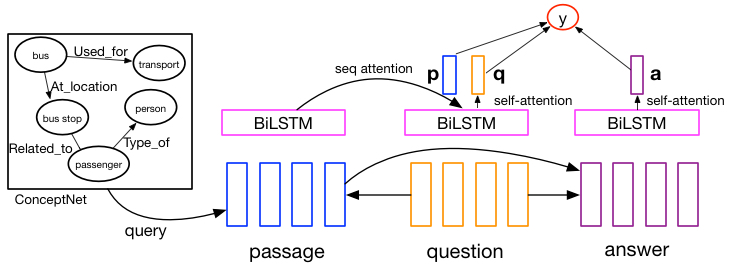
\includegraphics[scale=0.5]{TriAN.jpg}
	\caption{Structure of the original network \cite[p.2]{Wang:2018}}
	\label{fig:dnn}
\end{figure*}
This system is a deep learning neural network consisting of six different layer types. First the inputs generated in the preprocessing phase go through three embedding layers, each corresponding to the passage, question and answer respectively. There are also pos-embedding, ner-embedding and rel-embedding layers. The pos embedding gets the passage's and the question's pos tags as its input, the ner embedding layer gets the passage's ner tags and the relation embedding gets the relationship vectors generated using the \textit{ConceptNet}.

The word embeddings' outputs are paired up (passage-question, answer-question, answer-passage) and go through a so called \textit{sequence attention layer}. The \textit{sequence attention layer} at its core uses the bmm function in pytorch which performs a batch matrix-matrix product of the input matrices. This way it "matches" the two inputs together.

The system uses dropouts after the embedding and \textit{sequence attention layer} layers to avoid over-fitting.

These layers are followed by three \textit{stacked bidirectional rnn layer}, each corresponding to the passage, question and answer respectively. It differs from the standard bidirectional rnn layer in one aspect: it can concatenate the hidden states of the rnn. Their inputs are sort of self explanatory. The passage's \textit{stacked bidirectional rnn layer} gets the passage's word embedding layer, the output of the \textit{sequence attention layer} for the passage-question input pair, the passage's pos and ner embedding layers, the word frequency tensor created with the wikiword package, and the two relation embedding layer's output. The question's \textit{stacked bidirectional rnn layer} expects the question's word and pos embedding outputs on its input. The answer's \textit{stacked bidirectional rnn layer's} inputs are the answer's word embedding output and  the output of the \textit{sequence attention layer} for the answer-question and the answer-question input pairs.

This layer implicitly uses a dropout rate for regularization.

